\documentclass{article}
\usepackage[margin=1in]{geometry}
\usepackage{siunitx}
\usepackage{amsmath}
\usepackage{graphicx}
\sisetup{per-mode=symbol}
\title{Specific \& Latent Heat Worksheet}
\author{}
\date{}
\begin{document}
\maketitle

\section*{Questions}

\begin{enumerate}
\item Figure~\ref{fig:molecules} shows three collections of molecules, labelled (a)--(c).  
One is a \textbf{solid}, one a \textbf{liquid} and one a \textbf{gas}.  
Which is which?

\begin{figure}[h]
  \centering
  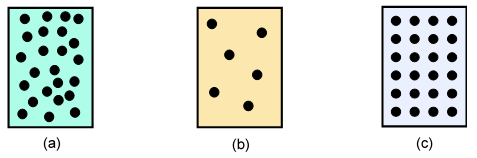
\includegraphics[width=0.7\linewidth]{figure1.png}% <-- put exported PNG here
  \caption{Collections of molecules (not to scale).}
  \label{fig:molecules}
\end{figure}

\item What happens to the molecules when a solid changes to a liquid?

\item What happens to the molecules in a solid when it is heated?

\item What is meant by the \emph{specific heat capacity} of a substance?

\item How much heat energy is needed to heat \SI{4}{\kilogram} of aluminium by \SI{80}{\celsius}?  
\textit{(Specific heat capacity of aluminium: \SI{1200}{\joule\per\kilogram\celsius})}

\item If \SI{48\,000}{\joule} of heat energy are given off when a \SI{2}{\kilogram} block of metal cools by \SI{120}{\celsius}, what is the specific heat capacity of the metal?

\item Water has a high specific heat.  Why is this useful when it is used as a coolant in engines?

\item Should saucepans be made of a material with a high or a low specific heat capacity?  Explain your answer.

\item A \SI{50}{\watt} heater is used to warm an aluminium block of mass \SI{5}{\kilogram}.  
After \SI{10}{\minute} the temperature of the block has risen by \SI{40}{\celsius}.  
Calculate  
  \begin{enumerate}
    \item the heat supplied by the heater;  
    \item the specific heat capacity of aluminium from these data;  
    \item why your answer differs from the accepted value in Question 5.
  \end{enumerate}

\item How much heat is given out when \SI{3}{\kilogram} of water at \SI{40}{\celsius} cool to \SI{25}{\celsius}?  
\textit{($c_\text{water} = \SI{4200}{\joule\per\kilogram\celsius}$)}

\item What temperature changes occur when ice changes to water at atmospheric pressure?

\item What happens to the molecules of a liquid when it is evaporating?

\item Why does your hand feel cold if you put a drop of methylated spirit on it?

\item How does sweating help to keep you cool?

\item A beaker of water is boiling on a Bunsen burner.  Describe carefully what happens when a few large spoonfuls of salt are added, and explain why.

\item Aerosol `freezers' are sold for cooling electronic components.  Do you think the molecules of the liquid inside evaporate easily?  Explain.

\item Top--class ice skaters are sometimes said to skate ``on water''.  Do you agree?  Explain.

\item Figure~\ref{fig:heatingcurve} shows how the temperature of a solid changes when it is heated steadily until it has turned into a gas.  
Identify the sections labelled A\,--\,E.

\begin{figure}[h]
  \centering
  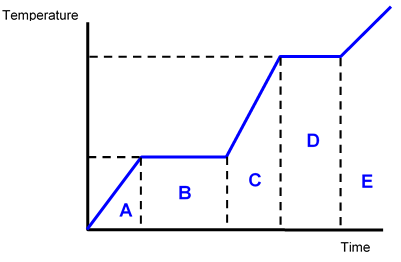
\includegraphics[width=0.75\linewidth]{figure2.png}% <-- put exported PNG here
  \caption{Heating curve for a substance.}
  \label{fig:heatingcurve}
\end{figure}

\item How much energy is needed to turn \SI{2}{\kilogram} of water at \SI{100}{\celsius} into steam at \SI{100}{\celsius}?  
\textit{(Latent heat of vaporisation of water: \SI{2.30e6}{\joule\per\kilogram})}

\item Explain what is meant by  
  \begin{enumerate}
    \item \textbf{specific latent heat of fusion};  
    \item \textbf{specific latent heat of vaporisation}.
  \end{enumerate}

\item How much heat energy is given out when \SI{500}{\gram} of steam at \SI{100}{\celsius} condense and cool to \SI{50}{\celsius}?

\item Why is a scald from steam at \SI{100}{\celsius} much more painful than one from water at \SI{100}{\celsius}?

\item Explain why snowballs cannot be made on very cold days.

\item How long will it take a \SI{50}{\watt} heater to melt \SI{2}{\kilogram} of ice at \SI{0}{\celsius}?  
\textit{(Latent heat of fusion of ice: \SI{3.35e5}{\joule\per\kilogram})}

\item Explain why the boiling point of water would be higher in a pressurised deep--sea diving bell than at the surface.

\end{enumerate}

\newpage
\section*{Answer Key}

\begin{enumerate}
\item (a) solid, (b) liquid, (c) gas.

\item The particles gain enough energy to break some of their fixed bonds, allowing them to move past one another while remaining close together.

\item They vibrate faster as they gain kinetic energy; if heated enough they overcome attractive forces and may melt.

\item The energy required to raise the temperature of \SI{1}{\kilogram} of a substance by \SI{1}{\celsius}.

\item $Q = mc\Delta T = 4 \times 1200 \times 80 = \SI{3.84e5}{\joule}$.

\item $c = \dfrac{Q}{m\Delta T} = \dfrac{48\,000}{2 \times 120} = \SI{200}{\joule\per\kilogram\celsius}$.

\item Because it can absorb large amounts of heat for only a small temperature rise, keeping engines near their optimum temperature.

\item Low specific heat capacity—so the pan itself warms quickly and transfers heat efficiently to the food.

\item 
  \begin{enumerate}
    \item $Q = Pt = 50 \times 600 = \SI{3.0e4}{\joule}$.  
    \item $c = \dfrac{Q}{m\Delta T} = \dfrac{3.0\times10^{4}}{5 \times 40} = \SI{150}{\joule\per\kilogram\celsius}$.  
    \item Energy was lost to the surroundings and the heater/heating leads, so not all of the electrical energy went into the block.
  \end{enumerate}

\item $Q = mc\Delta T = 3 \times 4200 \times 15 = \SI{1.89e5}{\joule}$ (released).

\item The temperature remains at \SI{0}{\celsius} until all the ice has melted; adding heat does not raise the temperature during the phase change.

\item Some molecules at the surface gain enough kinetic energy to overcome attractive forces and escape into the gas phase.

\item The spirit evaporates rapidly, taking latent heat from your skin, which lowers the skin temperature.

\item Sweat absorbs latent heat from the body as it evaporates, cooling the skin and the blood near the surface.

\item The boiling temporarily stops while the salt dissolves; the boiling point rises, so the water must reach a higher temperature before vigorous boiling resumes.

\item Yes.  The liquid must have a very low boiling point so that it vaporises easily, absorbing a lot of heat and producing a rapid cooling effect.

\item Largely true.  High pressure under the blade and frictional heating melt a thin layer of ice, providing a lubricating film of water on which the skater glides.

\item A: solid warming; B: melting plateau (solid $\rightarrow$ liquid); C: liquid warming; D: boiling plateau (liquid $\rightarrow$ gas); E: gas warming.

\item $Q = mL = 2 \times 2.30\times10^{6} = \SI{4.60e6}{\joule}$.

\item 
  \begin{enumerate}
    \item Energy required to melt \SI{1}{\kilogram} of a substance at its melting point.  
    \item Energy required to boil \SI{1}{\kilogram} of a substance at its boiling point.
  \end{enumerate}

\item Condensation: $Q_{1}= mL = 0.5 \times 2.30\times10^{6} = \SI{1.15e6}{\joule}$\\
      Cooling water: $Q_{2}= mc\Delta T = 0.5 \times 4200 \times 50 = \SI{1.05e5}{\joule}$\\
      Total $Q = \SI{1.26e6}{\joule}$ released.

\item Steam must first condense, releasing a large amount of latent heat, in addition to the heat needed to cool the water; water alone releases only the sensible heat.

\item The snow is too cold to partially melt and refreeze; without a thin film of water acting as ``glue'', the snow will not stick together.

\item $Q = mL = 2 \times 3.35\times10^{5} = \SI{6.70e5}{\joule}$\\
      $t = Q/P = 6.70\times10^{5} / 50 = \SI{1.34e4}{\second} \approx \SI{3.7}{\hour}$.

\item Increasing the pressure raises the boiling point, so water remains liquid at temperatures well above \SI{100}{\celsius} inside the diving bell.
\end{enumerate}

\end{document}
